\CHAPTER{DC readout performance and noise couplings}
\label{chapter5}
%\doublespace

The coupling of noises from the laser source and RF oscillators to the
gravitational wave readout channel differ considerably in RF and DC
readouts.  In addition, DC readout with an OMC is generally much more
sensitive to beam motion (jitter).  These couplings are of primary
interest in designing the optical readout of a gravitational wave
detector.

Furthermore we should verify that the touted sensitivity improvements
of DC readout are realized.

In this chapter, I will sketch the technique for calculating expected
noise couplings analytically and numerically, and I will present
measurements of these noise coupling measurements made on the two
Enhanced LIGO interferometers.

\SECTION{Sensitivity}

The primary figure of merit of a gravitational wave detector is its
noise floor, calibrated as a strain spectral density.  When evaluating
DC readout in Enhanced LIGO, we can begin by looking at the noise
floor: was the promised sensitivity delivered?  For the readout, the
answer is a resounding yes.  Given the input power and other known
parameters of the interferometer, the noise floor is accurately
modeled.

The shot-noise-limited sensitivity of a power-recycled interferometer
is given by a small number of parameters:

\begin{itemize}
\item the length of the arm cavities ($L = 3995$ m)\\
or, equivalently, the free spectral range ($\nu_0 = c/(2L)$)
\item the input power to the interferometer ($P_{IN}$)
\item the power recycling gain ($g_{cr}^2$)
\item the arm cavity finesse ($\mathcal{F} = 220$)
\item the input and output efficiency ($\epsilon$)
\item the laser wavelength ($\lambda = 1064\times10^{-9}$ m)
\end{itemize}
where we lump all losses due to absorption, scattering, or imperfect
mode-matching, and the photodiode quantum efficiency, into the efficiency
$\epsilon$.

The predicted curve is produced by dividing the amplitude spectral density of
the shot noise on the detection photodiode ($A_{shot})$ by the optical gain of
the interferometer ($S_{DC}$). The optical gain is (as derived earlier) simply
the derivative of the power at the output port with respect to changes in
differential arm length, evaluated at the operating DARM offset.
%
\begin{align}
A_{shot}(f) &= \sqrt{2 h (c/\lambda) P_{AS}} \\
S_{DC}(f) &= 2 \sqrt{\epsilon P_{IN} P_{AS}}\ g_{cr}^2\ r_{cp}\ \left(1 + i f/f_c\right)^{-1}
\end{align}
%
where $f_c = \nu_0 / (2\mathcal{F})$ is the cavity pole, $h$ is Planck's
constant, and $c$ is the speed of light.  This expression for $S_{DC}$ is in the single-pole
approximation, which is valid for frequencies much lower than the arm cavities'
free spectral range ($f\ll \nu_0)$, and for frequencies above the test mass
suspension's pendulum resonance (which may be increased due to radiation
pressue).

Combining these two expressions gives the noise floor due to shot noise,
calibrated in meters; dividing by $L$ gives the noise floor in strain:
%
\begin{align}
x_{shot}(f) & = \sqrt{\frac{h c}{2\ \lambda\ \epsilon\ P_{IN}}}\ \frac{1}{g_{cr}^2\ r_{cp}}
\ \left|1 + i \frac{f}{f_c}\right| \\
h_{shot}(f) &= (1/L)\ x_{shot}(f)
\label{eq:expected-shot-noise}
\end{align}
%
The shot noise seen at the photodiode has a white spectrum; the entire shape of
the shot noise when calibrated as a displacement or strain comes from the
calibration (i.e. the optical gain) which in turn is shaped only by the cavity
pole.  Interferometers using signal recycling will have a more complicated
response function.

\subsection{Measured and expected sensitivity}
The measured detector noise floors, calibrated as a displacement amplitude
spectral density ($m/\sqrt{\text{Hz}}$), along with the expected performance
based on equation~\ref{eq:expected-shot-noise} and measured detector parameters,
are depicted in figure~\ref{fig:shot-noise-limited-sensitivity}.  The measured
spectra were taken near the time of the detectors' highest inspiral ranges in
summer 2010.  The parameters used in the model are given in
table~\ref{tab:ifo-properties}.  

The comparison reveals that the achieved performance is as expected.  However,
some comments are in order: The H1 detector was able to operate with about twice
as much input power as the L1 detector, and had a power recycling gain
approximately 40\% better than L1's; from this we would expect considerably
better shot noise level at H1.  However, the H1 detector also experienced
anomalously low transmission of the arm cavity mode through the output mode
cleaner which contributed to a power efficiency ($\epsilon$) much lower than
desired.  The poor OMC transmission was due to some combination of poor
mode-matching, and high cavity losses which appeared near the end of the science
run.  These anomalous losses are not understood and are, as of the time of
writing, under active investigation.  

\begin{figure}
\includegraphics[width=\columnwidth]{figures/L1-965543700-thesis.pdf}
\includegraphics[width=\columnwidth]{figures/H1-962268780-thesis.pdf}
\caption[Shot noise sensitivity limit (measured and expected)]{\label{fig:shot-noise-limited-sensitivity}Shot noise limited sensitivity of the Livingston and Hanford detectors.}
\end{figure}



%% Cavity properties [Table]
% These values are all from Sam's document T080144:
% https://dcc.ligo.org/cgi-bin/private/DocDB/ShowDocument?docid=5416
\begin{table}
\centering
\begin{tabular}{l l l l l}
\hline 
\textbf{parameter}          &\textbf{Hanford}&\textbf{Livingston}  \\
\hline
arm cavity phase gain       & 137            & 137         \\
input optics efficiency     & 0.82           & 0.75        \\
interferometer mode-matching&                & 0.92        \\
carrier recycling gain      & $59\pm6$       & 41          \\
modulation depth            & 0.34           & 0.33        \\
OMC transmission            & 0.97           &             \\
OMC mode-matching           & 0.70           & 0.95        \\
Output Faraday transmission & $0.94\pm0.02$  & 0.9805      \\
DC-readout path pickoff     & 0.953          & 0.972       \\
PD quantum efficiency       & 0.98           &             \\
\hline
\end{tabular}
\caption{Designed and measured properties of the Hanford and Livingston interferometers.}
\label{tab:ifo-properties}
\end{table}


\SECTION{Laser and oscillator noise coupling mechanisms}

For the purpose of computing the frequency response of the interferometer and
the expected laser and oscillator noise couplings, it is convenient to regard
the electric field at any given location in the interferometer as a comb of
discrete spectral lines.  Generically, we refer to any spectral line as a
`sideband'.  The sidebands are divided into radio-frequency (RF) sidebands and
audio-frequency (AF) sidebands. The distinction is not actually the frequency of
the lines but their magnitude; RF sidebands have some finite amplitude, while
audio-frequency sidebands are infinitessimal.  When the electric field is
incident upon a photodiode, the photodiode will see a beat signal between every
pair of sidebands.  In our formalism we make the approximation that the product
of any two audio-frequency sidebands is zero.  Audio-frequency sidebands are
used simply as test fields to evaluate linear transfer functions.  They produce
signals at PDs by beating against the finite-amplitude RF sidebands.

As detailed in the preceeding chapter, the state of the LIGO interferometer is
determined by sampling the electric field at various ports using photodiodes.
Pairs of RF sidebands at several distinct frequencies are introduced at the
input to the interferometer; interference between these various fields allows
the state of the interferometer to be determined.  Around the laser carrier,
there are two pairs of RF sidebands, each produced through phase modulation: the
\emph{resonant sideband} at $\sim$25 MHz, which enters the interferometer and
emerges at the output port; and the \emph{non-resonant sideband} at $\sim$61
MHz, which is mostly reflected by the power recycling mirror.

For an intuitive understanding of the noise couplings to DC readout, we will
consider only the resonant sideband, an ignore the residual non-resonant
sideband.  In numerical simulations, both are included.  The arrangement of RF
sidebands is depicted in figure~\ref{fig:af-sidebands}.

Sidebands are typically created in pairs around a modulated the parent field;
and, when incident on a photodiode, they are most conveniently treated in pairs
too.  Instead of considering the amplitudes of upper and lower sidebands
separately, we can instead use a basis where we quantify the sidebands as some
amount of amplitude modulation (AM) and some amount of phase modulation.

\begin{figure}[]
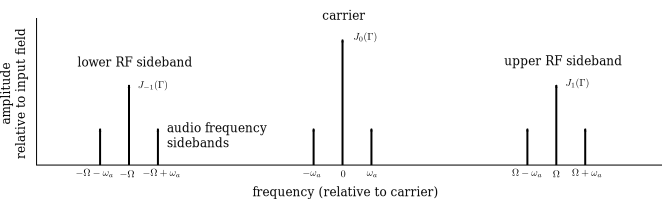
\includegraphics[width=\columnwidth]{figures/af_sidebands.pdf}
\label{fig:af-sidebands}
\caption{Schematic diagram of the laser carrier and RF sidebands, and their
  associated audio-frequency sidebands.}
\end{figure}

\SUBSECTION{Laser noises}

The Michelson-based design of laser interferometer gravitational wave detectors
is attractive due to its high common mode noise rejection.  A Michelson
interferometer with identical arms would completely isolate the output port from
common-mode noises (i.e. noise introduced at the input port).  Any asymmetries
between the arms will introduce couplings of noises at the input port to the
output port.  Some such asymmetries are unintentional, such as the difference in
finesse or reflectivity of the arms; intentional DARM and MICH asymmetries are
introduced in order to allow the local oscillator (RF or carrier) to read the
output port.

\subsubsection{Laser intensity noise}

Coupling of laser intensity noise to the output port is one of the easiest
couplings to understand.  The dominant mechanims (in the absence of radiation
pressure effects) are:
%
\begin{itemize}
\item Below the coupled-cavity pole ($f_{cc}\approx 1$ Hz), carrier power
  fluctuations are transmitted directly to the output port, attenuated only by
  the ratio $P_{AS}/P_{IN}$.  Above the coupled cavity pole, transmission of AM
  on the carrier is attenuated by $1/f$.
\item The resonant RF sidebands and any modulation they carry reaches the output
  port attenuated only slightly, since the Michelson is arranged (via the
  Schnupp asymmetry) to conduct the RF sidebands to the output port.  Because
  the RF sidebands are not resonant in the arms, noise on the RF sidebands is
  not attenuated by the coupled-cavity pole; instead they see a much lower
  finesse power recycling cavity and transmission is essentially flat in the
  band of interest.  Once reaching the output port, however, the RF sidebands
  are strongly attenuated by the OMC.
\end{itemize}
At low frequency, the carrier contribution dominates; at higher
frequency the residual RF sidebands dominate.  This is depicted in
figure~\ref{fig:laser-AM-contributions}.

\begin{figure}
\includegraphics[width=\columnwidth]{notes/figures/srcam_contributions.pdf}
\caption[Components of laser intensity noise contribution to DC readout]{\label{fig:laser-AM-contributions}Direct contributions of
  amplitude modulation of the laser carrier and RF sidebands to DC
  readout, in the absence of radiation pressure.  The carrier
  contribution is shaped by the coupled cavity pole.  The RF
  contribution is due to residual off-resonance transmission through
  the OMC.  Interference between the two coupling mechanisms creates a
  dip in the total coupling at the crossover frequency.}
\end{figure}

Laser intensity noise creates a varying radiation pressure force in the arm
cavities, which in turn causes displacement noise.  To distinguish this effect
from the inherent \emph{quantum} radiation pressure
noise\cite{Caves1980QuantumMechanical}, we refer to this as \emph{technical}
radiation pressure noise.  For identical arm cavities, the effect would be
entirely common mode.  Differences in arm cavity finesse and (especially) the
intentional differential detuning of the arm cavities produce a (potentially
large\cite{ChaibiOptomechanical}) coupling of technical radiation pressure noise
to DARM.

\subsubsection{Laser frequency noise}

\SUBSECTION{Oscillator noises}
%
Reduced coupling of noises from the RF oscillator is one of the
motivations for implementing DC readout. Despite not relying on the RF
sidebands directly, behavior of the RF oscillator is still able to
enter into the DC readout signal through control loop cross-couplings,
leakage of RF sideband power through the OMC, and amplitude modulation
of the laser carrier induced via AM on the RF oscillator.

\subsubsection{Oscillator AM}

Amplitude fluctuations of the RF oscillator produce a fluctuating modulation
depth; when the RF oscillator signal fluctuates upwards, more power is diverted
from the carrier into the RF sidebands.  The result is somewhat similar to laser
AM, except that carrier AM and RF AM are anti-correlated instead of correlated.

Unlike laser AM, oscillator AM does not produce equal relative intensity noise
(RIN) variations of the carrier and sidebands; this is simply because oscillator
AM results in equal and opposite changes of power in the carrier and sideband
rather than linear scalings of both.  The sideband RIN per oscillator AM is
given by
\begin{equation}
\frac{\text{SB RIN}}{\text{OSC AM}}=2\Gamma_{0}\frac{J_{1}'(\Gamma_{0})}{J_{1}(\Gamma_{0})}=\Gamma_{0}\frac{J_{0}-J_{2}}{J_{1}}
\end{equation}
%(see Livingston elog 2010-07-15, {}``sideband RIN per oscillator AM calculation,'' ).
where $\Gamma_0$ is the nominal modulation depth, $J_n(z)$ is the $n$th Bessel
function, and $J_n'(z)=(\partial/\partial z)J_n(z)$ is the derivative of the Bessel function.

Measured coupling is shown in figure \ref{fig:oscillator-AM-coupling-measured}.

\subsubsection{Oscillator phase noise}

Phase noise on the RF oscillator produces phase noise on the resulting RF
sidebands, but does not affect the laser carrier.  Its direct coupling to DC
readout is therefore quite small; to couple to DC readout, the phase noise
sidebands must be converted to AM through Michelson asymmetries, and then
survive attentuation by the OMC.

\section{Laser and oscillator noise coupling measurements}

Laser and oscillator noise couplings were measured at both the H1 and
L1 detectors\footnote{Measurements at Hanford were made by Nicol\'as
  Smith.}, at a selection of DARM offsets.  In this section I explain
how the measurements were made and discuss the results.

\subsection{Laser noise coupling measurements}

The LIGO laser source contains an intensity stabilization servo (ISS)
which reduces the relative intensity noise (RIN) of the laser power
before the laser enters the interferometer.  Injecting an excitation
into the error point of this servo impresses intensity noise onto the
beam.  The laser intensity noise coupling was measured by taking
synchronous swept-sine transfer functions from a monitor photodiode
just after the ISS and the DARM readout.

\begin{figure}[]   % Laser AM
\includegraphics[]{figures/laserAM-L1.pdf}
\includegraphics[]{figures/laserAM-H1.pdf}
\caption[Laser intensity noise coupling (measured and modeled)]{Laser intensity noise coupling to DARM.
  Solid lines are the results of a frequency-domain, plane-wave model; dotted lines are linear transfer function measurements.  Color represents the DARM offset, with warm colors for positive offsets and cool colors for negative offsets.  The upper plot is Livingston; the lower one is Hanford.}
\end{figure}

The laser frequency is stabilized to the mean length of the two arms
(CARM) by a high-bandwidth analog servo, the common mode servo.
Frequency modulation can be induced by injecting into the error point
of this servo.  Unlike with the ISS, there is no separate witness
sensor to provide a direct measurement of the induced laser frequency
modulation.  Instead we must make a calibration of the common mode
servo error point.  The frequency noise coupling is to be calibrated
in terms of Hz of frequency noise \emph{before} the stabilizing action
of the common mode servo, so we must account for the suppression of
the loop.  The calibration was done by porting the calibration of DARM
to CARM, as follows:

\begin{enumerate}
\item Drive the position of one of the end test masses (ETMs) with a
  sinusoidal modulation at some probe frequency ($f=7300$ Hz was
  used).  In the absence of loops, this would produce equal DARM and
  CARM motion.
\item Measure the response in the DARM and CARM readouts.  The CARM
  readout channel is REFL\_I, which senses the mismatch between the
  laser carrier frequency and the CARM length.
\item Apply the DARM calibration.  This includes compensation for the
  DARM control loop.
\item Compensate for the frequency noise suppression of the common
  mode loop by multiplying by $1+G$ where $G$ is the (complex) open
  loop gain of the common mode loop at the probe frequency.
\item Equate the calibrated DARM and loop-corrected CARM.  This gives
  a calibration for CARM in meters at the probe frequency.
\item Multiply by $\delta\nu/\delta L = \nu/L = c/(\lambda L)$ to
  convert from meters to Hz.
\item Assume a model for the CARM to REFL\_I transfer function to
  propagate the calibration to other frequencies.  This transfer
  function is simply the coupled-cavity pole\cite[eq. 3.5]{RanaThesis}.
\end{enumerate}

\begin{figure}
\includegraphics[]{figures/laserFM-L1.pdf}
\includegraphics[]{figures/laserFM-H1.pdf}
\caption[Laser frequency noise coupling (measured and modeled)]{Laser frequency noise coupling to DARM}
\end{figure}

\subsection{Oscillator noise coupling measurements}

To measure oscillator noise couplings we temporarily switched the
source of the 25 MHz oscillator from the Wenzel crystal oscillator to
a general purpose (IFR 2023A) RF function generator, which accepts
phase and amplitude modulation inputs.  The measurements were made by
connecting a spare DAC output to the modulation input of the IFR
function generator and then taking synchronous swept-sine transfer
functions from the modulation drive to the DC readout with the
interferometer in its running configuration.

To calibrate the oscillator AM transfer function, we configured the
interferometer optics (by misaligning unneeded mirrors) to send a
fraction of the input light directly to the OMC and locked the OMC to
one of the RF sidebands.  Taking the transfer function in this
configuration allowed a direct measurement of the AM imposed on the RF
sidebands\footnote{Thank you to Robert Ward for suggesting the
  technique.}.  To calibrate the oscillator PM transfer function, a
curve with the same shape as the AM calibration was used, but with the
DC value determined by the front panel setting of the phase modulation
depth on the function generator.  This was checked separately at a few
individual frequencies by connecting the output of the function
generator directly to an RF spectrum analyzer.

\begin{figure} % Oscillator AM
\includegraphics[]{figures/oscAM-L1.pdf}
\includegraphics[]{figures/oscAM-H1.pdf}
\caption[Oscillator amplitude noise coupling (measured and modeled)]{\label{fig:osc-AM}Oscillator amplitude noise coupling to DARM}
\end{figure}

\begin{figure} % Oscillator PM
\includegraphics[]{figures/oscPM-L1.pdf}
\includegraphics[]{figures/oscPM-H1.pdf}
\caption[Oscillator phase noise coupling (measured)]{\label{fig:osc-PM}Oscillator phase noise coupling to DARM.}
\end{figure}

\SECTION{Beam jitter noise}
%
Beam jitter noise is perhaps the most important new noise source in
DC readout and is tied to alignment of the OMC, which has proved to
be one of the most subtle new issues. The output mode cleaner converts
motion of the input beam into variations in transmission. The resulting
variation in the transmitted light level is indistinguishable from
DARM motion.



\SECTION{Electronics noise}
%
An optical power of 100 mW on the readout photodiodes will produce a
photocurrent of $i = q_e\lambda/(hc)\cdot 100\text{ mW } = 86\text{ mA}$, which
in turn has a shot noise floor of $\sqrt{2 q_e i}\approx 500 \text{
  pA}/\sqrt{\text{Hz}}$.  Across $100\ \Omega$ transimpedance, this becomes $50
\text{ nV}/\sqrt{\text{Hz}}$.  The noise floor of the readout electronics must
be below this level and not be polluted by any baseband $1/f$ flicker noise.

The main strategy is to aggressively amplify the electronic signal as close to
the photodiodes as possible, so that noises added downstream become
insignificant.  To eliminate even triboelectric effects, the first preamp stages
are placed in-vacuum.  The in-vacuum preamps consist of active filter stages
with two zeros at 8 Hz and two poles at 80 Hz, for a factor of 100 amplification
at 100 Hz.  This is followed by two more pole-zero pairs in satellite amplifiers
on the floor outside the vacuum chamber, for a total gain of 10,000 before the
long run to the racks.

\begin{comment}
h = 6.626068e-34;
c = 299792458;
lambda = 1064e-9;
qe = 1.60217646e-19;
I = qe * lambda / (h * c)
sqrt(2* qe * I)
\end{comment}

\SECTION{Optical spring}
%
Detuning the arm cavities from their resonance introduces a big optical
spring.

\begin{equation}
k_{opt}\approx\frac{64\mathcal{F}^{2}g^{2}P_{IN}}{c\lambda^{2}}\left(\delta x\right) 
\end{equation}

\SECTION{Technical radiation pressure noise}

Amplitude noise on the input laser field produces modulation radiation
pressure on the optics, in particular in the arm cavities.  If the arm
cavities were identical, this coupling would be entirely common mode.
However, once the arms are differentially detuned, the radiation
pressure noise attains a differential component.

We can treat the radiation pressure noise as a displacement noise.

Suppose the arm cavities are initially identical, with all 
suspensions having resonant frequency $\omega_0$.  The optical spring
shifts this resonance to $\omega_0 \pm \delta\omega$.

The intensity noise to displacement transfer function is
\begin{equation}
  P_{IN} {g_{rc}}^2 {g_{cav}}^2 \frac{1}{s_{cc}} 
\end{equation}

\SECTION{Nonlinearity  of the DC error signal}
%
Although we operate sufficiently far from the dark fringe that the
linear coupling of residual DARM motion to output power is dominant,
sufficiently large motion could produce second-order coupling. Fortunately,
this turns out to be totally negligible.

\SECTION{Optical gain}

\SECTION{Digital effects}

The realtime digital signal processing system through which our
control systems are implemented provide the illusion of a continuous,
analog system.  However, it is important to remember that the
underlying system operates on quantized values in discrete time in
order to avoid being caught by surprise by ``digital noises''.

\begin{itemize}
\item Finite, non-deterministic execution time
\item ADC bit noise
\item Floating point dynamic range
\item Synchronized communications
\end{itemize}
